% Part 1: Evolutionary Pathways of Large Language Models
\section{Evolutionary Pathways of Large Language Models}

\begin{frame}
\frametitle{Transformer Architecture}
\begin{itemize}
    \item \textbf{"Attention is All You Need"} (Vaswani et al., 2017)
    \item Self-attention mechanism: captures long-range dependencies
    \item Key components:
    \begin{itemize}
        \item Multi-head attention
        \item Positional encoding
        \item Feed-forward networks
        \item Layer normalization
    \end{itemize}
    \item Technical evolution of transformer architectures:
    \begin{itemize}
        \item Dense Attention $\rightarrow$ MQA $\rightarrow$ GQA $\rightarrow$ MLA $\rightarrow$ DSA
        \item Dense FFN $\rightarrow$ MoE
        \item Towards fine-grained MoE specialization
    \end{itemize}
\end{itemize}
\end{frame}

\begin{frame}
\frametitle{Probabilistic Modeling}
\begin{itemize}
    \item Word-level probability prediction: $P(w_1, w_2, ..., w_n)$
    \item Current training paradigms:
    \begin{itemize}
        \item Autoregressive language modeling
        \item Diffusion models
    \end{itemize}
    \item Training methods: Pre-training, SFT, DPO, PPO, GRPO
    \item Trends:
    \begin{itemize}
        \item From expert knowledge to autonomous exploration
        \item From off-policy to on-policy learning
    \end{itemize}
\end{itemize}
\end{frame}

\begin{frame}
\frametitle{Scaling Laws}
\begin{columns}
\column{0.5\textwidth}
\begin{itemize}
    \item Power law relationship:
    \begin{equation*}
    L(N, D, C) \approx A N^{-\alpha} + B D^{-\beta} + E
    \end{equation*}
    \item \textbf{Key variables}:
    \begin{itemize}
        \item $N$: Model size (parameters)
        \item $D$: Dataset size (tokens)
        \item $C$: Compute budget (FLOPs)
    \end{itemize}
    \item Optimal compute allocation strategies
\end{itemize}
\column{0.5\textwidth}
\begin{center}
\includegraphics[width=0.7\textwidth]{images/scaling_law.pdf}
\end{center}
\end{columns}
\end{frame}

\begin{frame}
\frametitle{Emergent Abilities}
\begin{itemize}
    \item Capabilities that appear at scale, absent in smaller models
    \item Key emergent behaviors:
    \begin{itemize}
        \item Few-shot learning
        \item Zero-shot learning
        \item Chain-of-thought reasoning
        \item ReAct loop (reasoning and acting)
        \item Interleaved thinking
    \end{itemize}
\end{itemize}
\end{frame}

\begin{frame}
\frametitle{LLM and Agent Development Roadmap}
\begin{center}
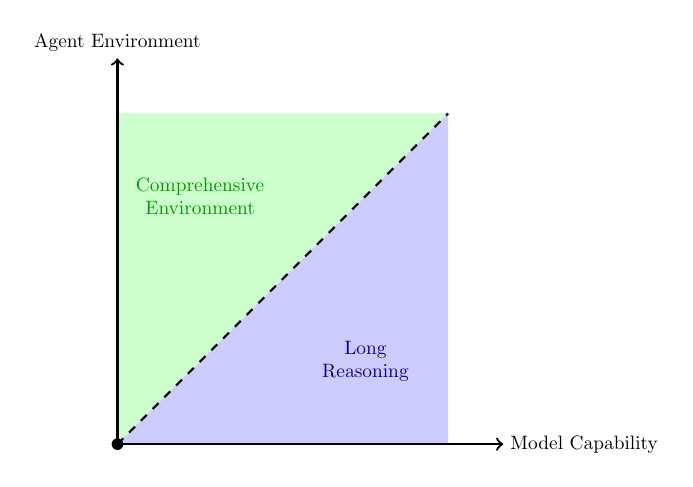
\begin{tikzpicture}[scale=0.7, every node/.style={scale=0.7}]
    % Define the size of the square
    \def\maxsize{6}
    
    % Fill upper-left triangle (Comprehensive Environment)
    \fill[green!20] (0,0) -- (0,\maxsize) -- (\maxsize,\maxsize) -- cycle;
    
    % Fill lower-right triangle (Long Reasoning)
    \fill[blue!20] (0,0) -- (\maxsize,0) -- (\maxsize,\maxsize) -- cycle;
    
    % Draw the diagonal line y=x
    \draw[thick, dashed] (0,0) -- (\maxsize,\maxsize);
    
    % Axes
    \draw[->, thick] (0,0) -- (\maxsize+1,0) node[right] {Model Capability};
    \draw[->, thick] (0,0) -- (0,\maxsize+1) node[above] {Agent Environment};
    
    % Origin point (without text label)
    \fill (0,0) circle (3pt);
    
    % Labels for regions
    \node[green!60!black, align=center] at (1.5,4.5) {Comprehensive\\Environment};
    \node[blue!60!black, align=center] at (4.5,1.5) {Long\\Reasoning};
\end{tikzpicture}
\end{center}
\end{frame}
